\documentclass[journal,12pt,twocolumn]{IEEEtran}
\usepackage{graphicx}
\graphicspath{{./figs/}}{}
\usepackage{amsmath,amssymb,amsfonts,amsthm}
\newcommand{\myvec}[1]{\ensuremath{\begin{pmatrix}#1\end{pmatrix}}}

\let\vec\mathbf

\title{
Matrix-Conics
}
\author{Kukunuri Sampath Govardhan}
\begin{document}
\maketitle
\tableofcontents
\bigskip

\section{Problem Statement}
\begin{flushleft}
In an Ellipse, the distance between its foci is 6 and minor axis is 8. Then find its Eccentricity.\\
\end{flushleft}
\section{Construction}
\begin{figure}[h]
    \centering
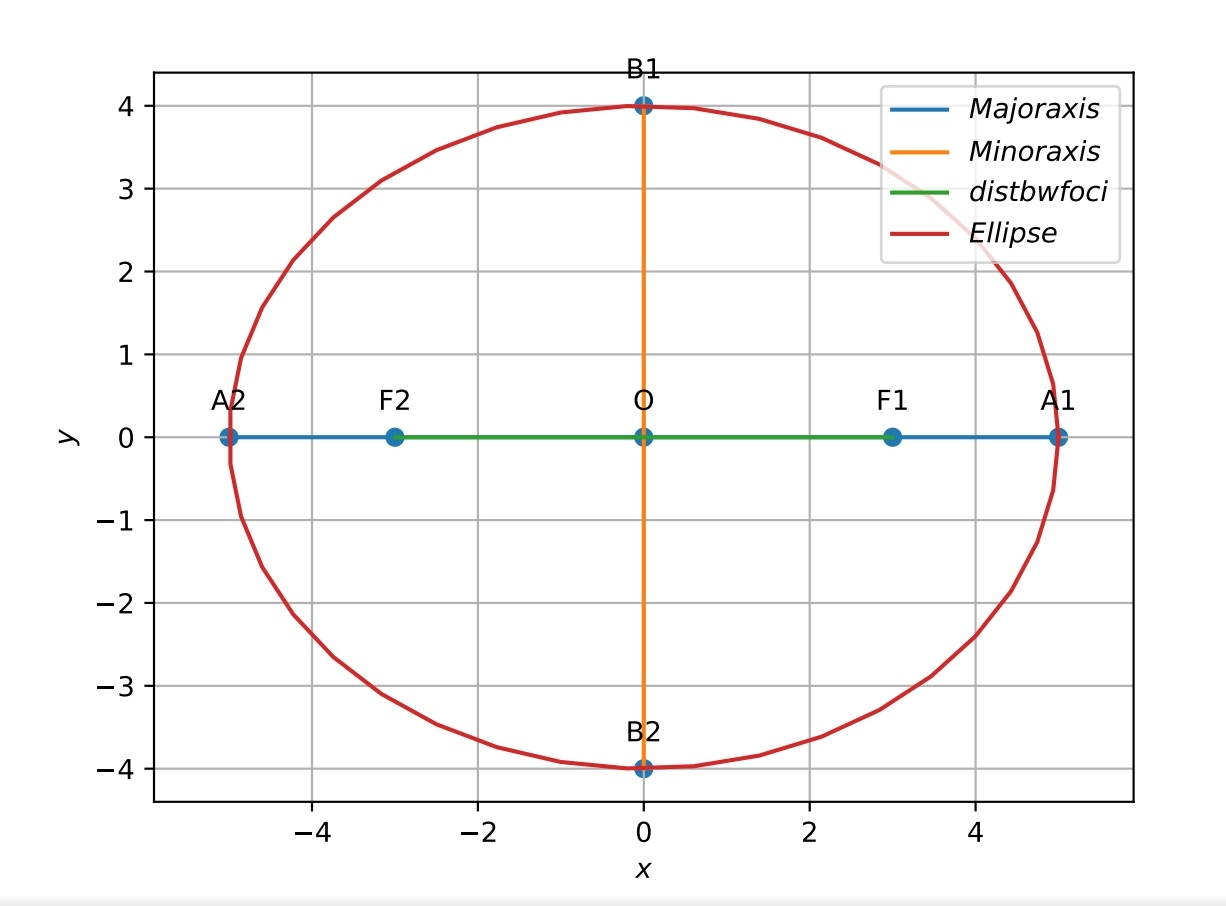
\includegraphics[width=\columnwidth]{figs/assign6.png}
    \caption{Ellipse}
    \label{fig:my_label}
\end{figure}
\begin{table}[h]
    \centering
    \begin{tabular}{|c|c|c|}
       \hline
       \textbf{Symbol}&\textbf{Value}&\textbf{Description}  \\
       \hline
            ${||\vec{F_1} - \vec{F_2}||}$ & 6 & Distance between foci\\
        \hline
            ${||\vec{B_1} - \vec{B_2}||}$ & 8 & Length of Minor axis\\
        \hline
        $\vec{e_1}$ & \myvec{1 \\ 0} & Standard Basis Vector \\
        \hline
        e & & Eccentricity \\
            \hline
    \end{tabular}
    \caption{Parameters}
    \label{tab:my_label}
\end{table}
\vspace{2cm}
\section{Solution}
The length of minor axis in ellipse is\\
\begin{equation}
        ||\vec{B_1} - \vec{B_2}|| = 2\sqrt{|\frac{f_0}{\lambda_2}|}\label{eq-1}
\end{equation}
Therefore,\\
\begin{center}
	8 = $2\sqrt{|\frac{f_0}{\lambda_2}|}$
\end{center}
Yielding,\\
\\
\begin{equation}
\frac{f_0}{\lambda_2} = 16 \label{eq-2}\\
\end{equation}
\\
The focal points \\
\begin{equation}
        \vec{F_1} =
        \frac{\frac{1}{e\sqrt{1 - e^2}}e^2\sqrt{\frac{\lambda_2}{f_0}}\vec{e_1}}{\frac{\lambda_2}{f_0}}
\end{equation}
\begin{equation}
        \vec{F_2} = -
        \frac{\frac{1}{e\sqrt{1 - e^2}}e^2\sqrt{\frac{\lambda_2}{f_0}}\vec{e_1}}{\frac{\lambda_2}{f_0}}
\end{equation}
\begin{center}
$||\vec{F_1} - \vec{F_2}|| = 2\frac{\frac{1}{e\sqrt{1 - e^2}}e^2\sqrt{\frac{\lambda_2}{f_0}}||\vec{e_1}||}{\frac{\lambda_2}{f_0}}$ \\
\vspace{0.3cm}
$6 = \frac{\frac{1}{\sqrt{1 - e^2}}e\sqrt{\frac{\lambda_2}{f_0}}}{\frac{\lambda_2}{f_0}}$
\end{center}
Substuting $\frac{\lambda_2}{f_0}$ from eq-2, \\
\begin{equation}
       6 = 2\frac{e}{\sqrt{1 - e^2}}\frac{1}{4}\frac{16}{1}
\end{equation}
 Yielding,   \\
 \begin{center}
	 $e = \frac{3}{5}$ 
 \end{center}
 Therefore,\\
\\
\begin{center}
$\boldsymbol{Eccentricity, e = \frac{3}{5}}$ 
\end{center}
\end{document}

